\section{RISMC approach to PRA}
\label{sec:rismc}
The RISMC approach~\cite{RISMC} employs both deterministic and stochastic methods 
in a single analysis framework (see Figure~\ref{fig:RISMCoverview}). In the deterministic method 
set we include:
\begin{itemize}
  \item Modeling of the thermal-hydraulic behavior of the plant~\cite{BWR_SBO_Mandelli,BWRanalysis}
  \item Modeling of external events such as flooding~\cite{mandelliPSA2015}
  \item Modeling of the operators’ responses to the accident scenario~\cite{HRA_BoringReport2014}
\end{itemize}

\begin{figure}
    \centering
    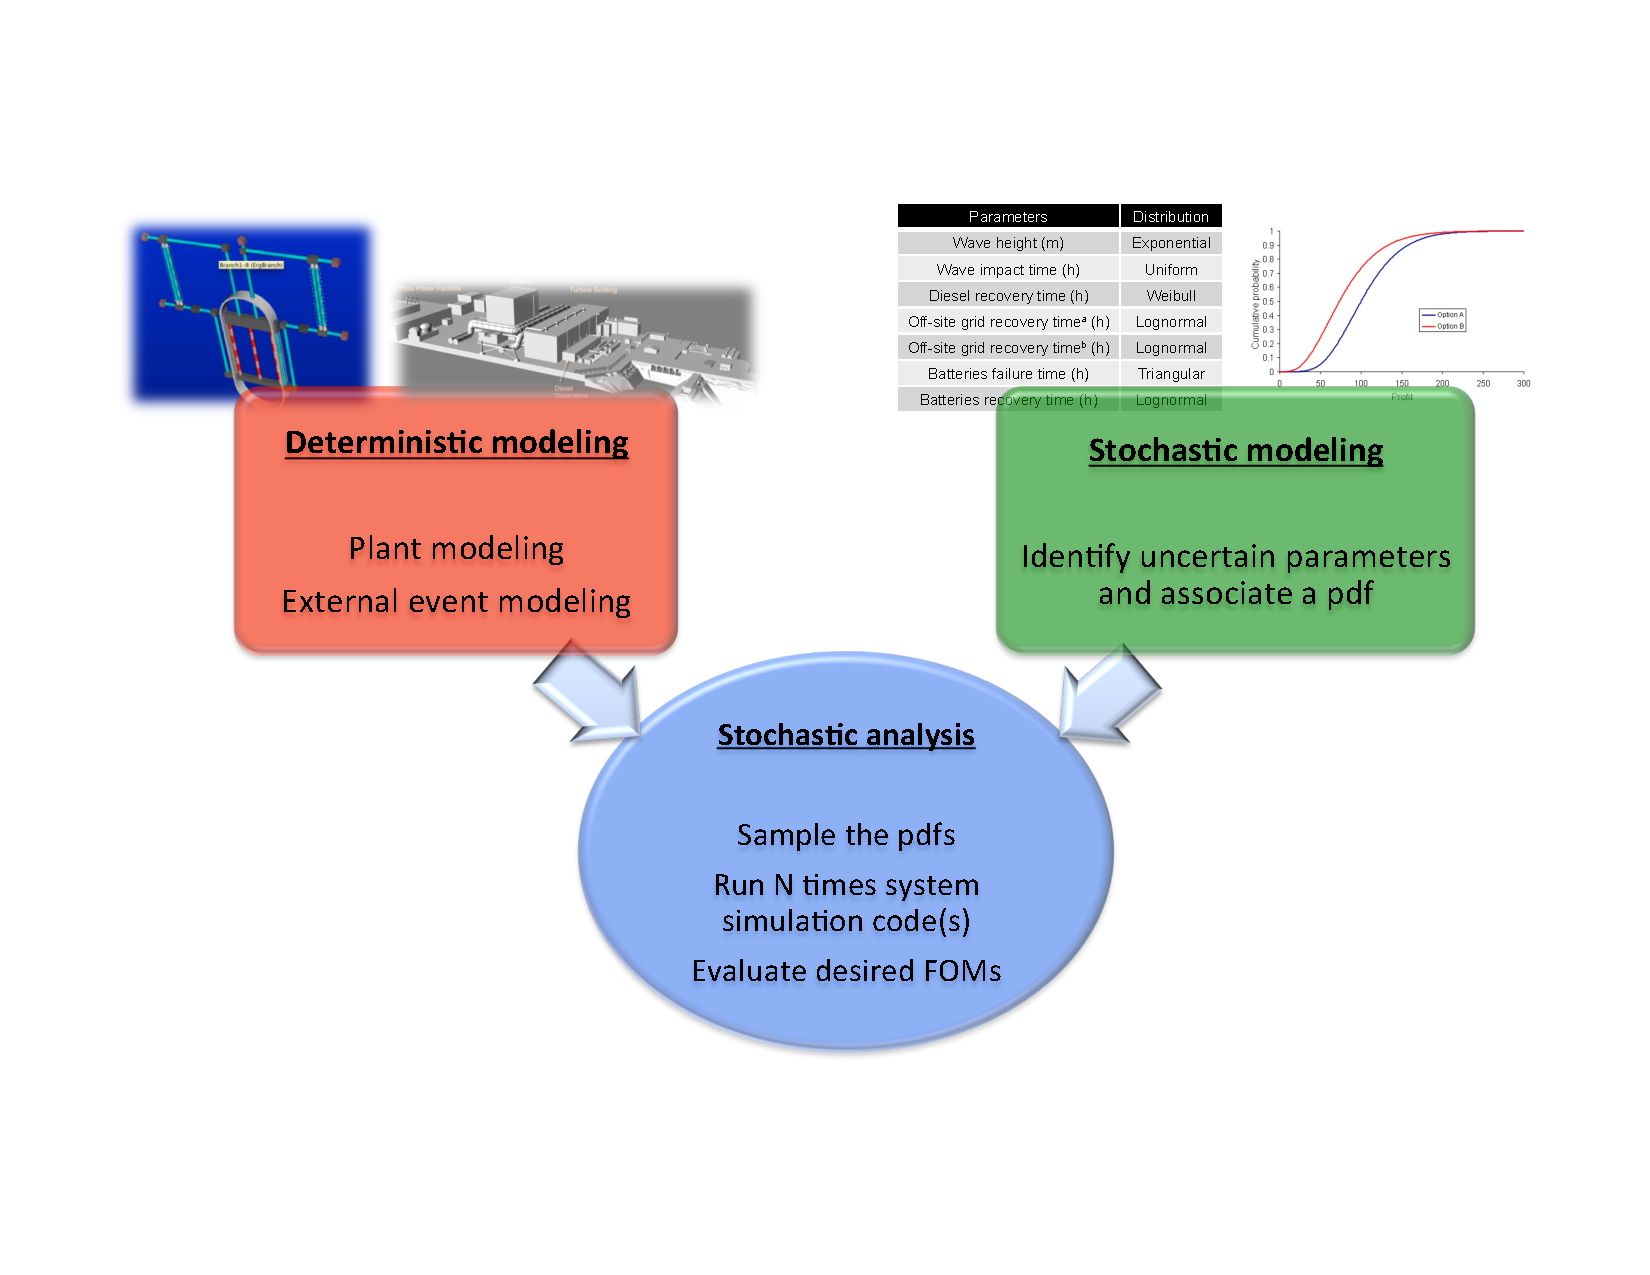
\includegraphics[scale=0.5]{RISMCoverview.pdf}
    \caption{Overview of the RISMC approach}
    \label{fig:RISMCoverview}
\end{figure}

Note that deterministic modeling of plant or external events can be performed by employing 
specific simulator codes but also surrogate models, known as reduced order models (ROM)~\cite{ROM_Khalik}. 
ROMs would be employed in order to decrease the high computational costs of employed codes.
In addition, multi-fidelity codes can be employed to model the same system; the idea is to 
switch from low-fidelity to high-fidelity code when higher accuracy is needed (e.g., use 
low-fidelity codes for steady-state conditions and high-fidelity code for transient conditions).

In stochastic modeling we include all stochastic parameters that are of interest in the PRA 
analysis such as:
\begin{itemize}
  \item Uncertain parameters
  \item Stochastic failure of system/components
\end{itemize}
As mentioned earlier, the RISMC approach heavily relies on multi-physics system simulator 
codes (e.g., RELAP5-3D~\cite{relap5}) coupled with stochastic analysis tools (e.g., RAVEN~\cite{RAVEN_PSAM_2014}). 

\subsection{System Modeling}

\subsection{Human Modeling}

\subsection{External Event Modeling}

\subsection{ROM Modeling}